\documentclass[multi=tikzpicture]{standalone}

\usepackage{tikz}
\usetikzlibrary{shapes.geometric, arrows}
\usepackage{varwidth}


\tikzstyle{startstop} = [rectangle, rounded corners, 
minimum width=3cm, 
minimum height=1cm,
text centered, 
draw=black, 
fill=red!30]

\tikzstyle{io} = [trapezium, 
trapezium stretches=true, % A later addition
trapezium left angle=70, 
trapezium right angle=110, 
minimum width=3cm, 
minimum height=1cm, text centered, 
draw=black, fill=blue!30]

\tikzstyle{process} = [rectangle, 
minimum width=3cm, 
minimum height=1cm, 
text centered, 
text width=3cm, 
draw=black, 
fill=orange!30]

\tikzstyle{decision} = [diamond, 
minimum width=3cm, 
minimum height=1cm, 
text centered,
draw=black, 
fill=green!30]
\tikzstyle{arrow} = [thick,->,>=stealth]

\begin{document}

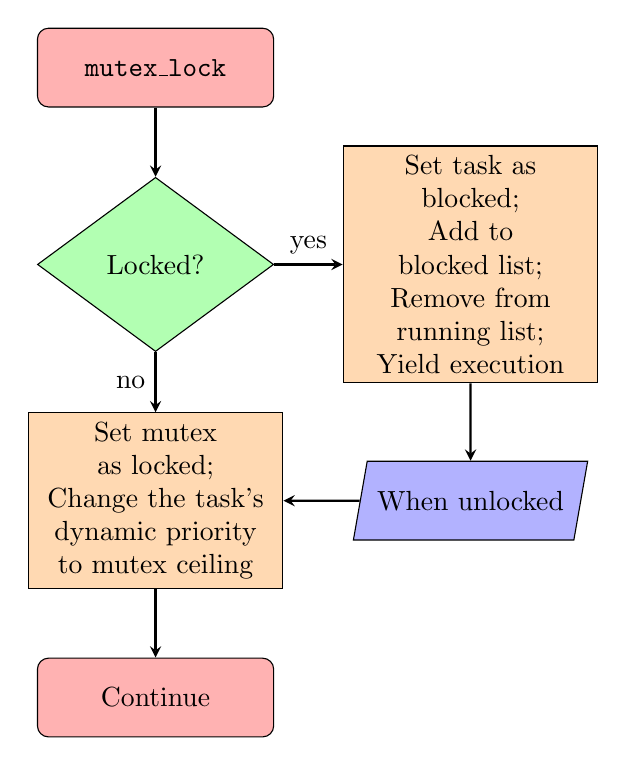
\begin{tikzpicture}[node distance=2cm]
    \node (start) [startstop] {\texttt{mutex\_lock}};

    \node (if_locked) [decision, below of=start, text width=1.5cm, yshift=-0.5cm] {Locked?};

    \node (lock) [process, below of=if_locked, yshift=-1cm] {Set mutex as locked;\\
    Change the task's dynamic priority to mutex ceiling};

    \node (block) [process, right of=if_locked, xshift=2cm] {Set task as blocked;\\
    Add to blocked list;\\
    Remove from running list;\\
    Yield execution};

    \node (unlocked) [io, below of=block, yshift=-1cm] {When unlocked};
    \node (end) [startstop, below of=lock, yshift=-0.5cm] {Continue};

    \draw [arrow] (start) -- (if_locked);
    \draw [arrow] (if_locked) -- node[anchor=east] {no} (lock);
    \draw [arrow] (if_locked) -- node[anchor=south] {yes} (block);
    \draw [arrow] (block) -- (unlocked);
    \draw [arrow] (unlocked) -- (lock);
    \draw [arrow] (lock) -- (end);
\end{tikzpicture}

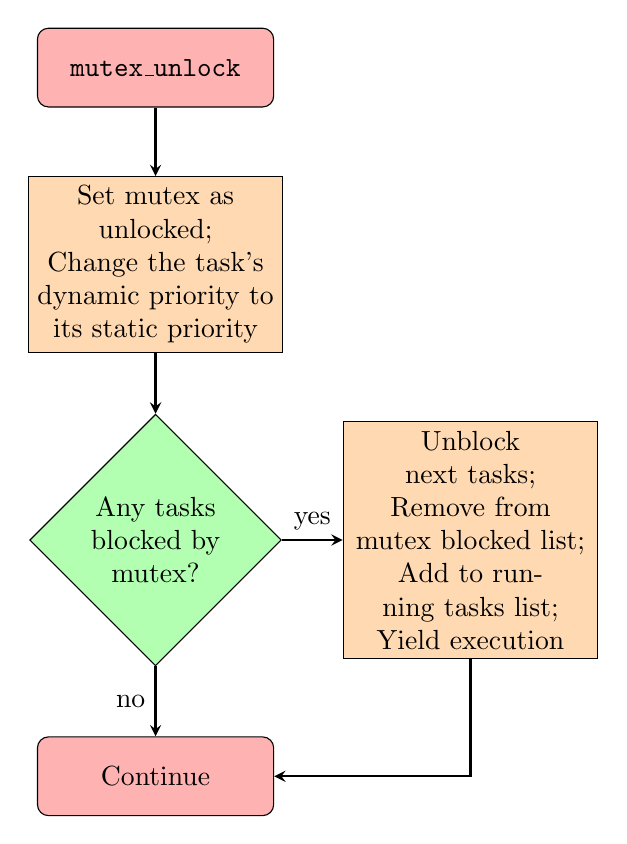
\begin{tikzpicture}[node distance=2cm]
    \node (start) [startstop] {\texttt{mutex\_unlock}};
    
    \node (unlock) [process, below of=start, yshift=-0.5cm] {Set mutex as unlocked;\\
    Change the task's dynamic priority to its static priority};

    \node (if_blocked) [decision, below of=unlock, yshift=-1.5cm] {\begin{varwidth}{2cm}\centering Any tasks blocked by mutex?\end{varwidth}};
    
    \node (unblock) [process, right of=if_blocked, xshift=2cm] {Unblock next tasks;\\
    Remove from mutex blocked list;\\
    Add to running tasks list;\\
    Yield execution};
    
    \node (end) [startstop, below of=if_blocked, yshift=-1cm] {Continue};
    
    \draw [arrow] (start) -- (unlock);
    \draw [arrow] (unlock) -- (if_blocked);
    \draw [arrow] (if_blocked) -- node[anchor=south] {yes} (unblock);
    \draw [arrow] (if_blocked) -- node[anchor=east] {no} (end);
    \draw [arrow] (unblock) |- (end);
    \end{tikzpicture}

\end{document}